\documentclass{article}
\usepackage{graphicx} % Required for inserting images
\title{Week 1 Journal}
\author{Abdul Shakur Illiyasu}
\date{\today}

\begin{document}
\maketitle

\begin{figure}[ht]
    \centering
    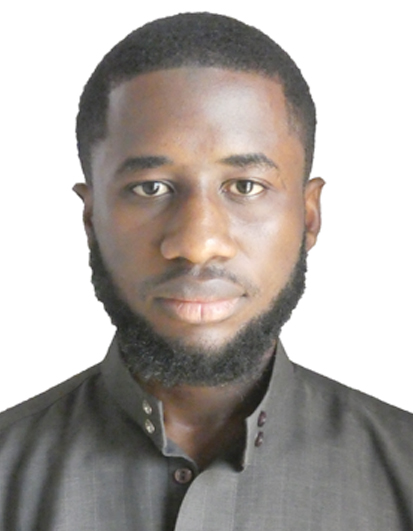
\includegraphics[width=0.35\textwidth]{abdul.jpg}
    \caption{Abdul Shakur Illiyasu}
    \label{fig: picture.jpg}
\end{figure}

\section{Goals and What I Hope to Learn}

My goal for CS6000 is to finish the semester as a better research student. I aim to strengthen my problem-solving and logical reasoning skills, particularly in breaking down complex problems. This course will prepare me for future research and improve my writing and presentation abilities.

As someone who transitioned directly from an undergraduate to a PhD program without research experience, I hope to learn the fundamentals of conducting good research, publishing quality papers, and critically evaluating research papers.

\subsection{Degree and Research Project}
I am pursuing a PhD in cybersecurity and will be conducting research under Dr. Change on the Mutual Randomness Project. This project involves image and depth camera sensing and processing, to extract randomness, information, and entropy. Like CloudFlare’s lava lamp-based entropy, this project focuses on the mutual randomness observed by two entities. It examines the relative positions, movements, and perspectives between these entities, which are expected to be highly correlated. The randomness and entropy generated will secure communication between the entities, equipped with cameras and mobility capabilities.

\subsection {Something Personal}
One of my core values is to help others without expecting anything in return. This mindset ensures that I avoid disappointment when someone is unable to reciprocate when I need help. By not expecting anything in return, I protect myself from potential disappointment, and this approach greatly influences how I manage my work and relationships.